\chapter{Resultados Experimentais}\label{chp:resultados}

Este capítulo discorre sobre os procedimentos realizados para a obtenção dos resultados comparativos da rmM-tree proposta por \citet{paper-fully-functinal-succint-trees},
com a rmM-tree k-ária proposta neste trabalho. O mesmo está dividido da seguinte forma: a seção~\ref{sec:base-de-dados} apresenta o conjunto de dados usado na avaliação experimental.
As seções seguintes apresentam as configurações da máquina usada para realizar os testes (Seção~\ref{sec:configuracao}), o modo como os mesmos foram realizados (Seção~\ref{sec:experimentos}),
e por últimos os resultados obtidos (Seção~\ref{sec:resultados}).


\section{Base de dados}\label{sec:base-de-dados}
Afim de realizar testes que comprovem o desempenho das estruturas implementadas na ptrática, usamos em nossos testes quatro conjuntos de dados do mundo real,
estes conjuntos estão disponíveis no endereço eletrônico \href{http://www.inf.udec.cl/~jfuentess/datasets/sequences.php}{www.inf.udec.cl}.
A tabela~\ref{tbl:dataset} mostra um resumo dos conjuntos usados, a primeira coluna da tabela refere-se ao nome do conjunto de dados,
a segunda coluna indica o tamanho do conjunto de dados em MB, a coluna de número 3 mostra a quantidade de parênteses do respectivo conjunto de dados.
A quarta coluna exibe a quantidade nós da árvore representada pela sequência de parêntesses fornecida,
e  por fim, a quinta coluna mostra o número de entradas usadas em nossos testes para cada conjunto de dados.


\begin{table}[!ht]
  \centering
  \caption[Conjunto de dados usados em testes experimetais]{Conjunto de dados usados nos testes experimetais }
  \label{tbl:dataset}
	\resizebox{\columnwidth}{!}{
        \begin{tabular}{|l|l|l|l|l|}
        \hline
        \textbf{Conjunto de dados}                       & \textbf{Tamanho (MB)}                      & \textbf{Quantidade de parênteses}                      & \textbf{Tamanho da árvore representada} & \textbf{Número de entradas usadas} \\ \hline
        Complete tree (ctree)                            & 18                                          & 2.147.483.644                                          & 1.073.741.822                           & 1.000.000                                               \\ \hline
        DNA                                              & 135                                         & 1.154.482.174                                          & 577.241.087                             & 100.000.000                                             \\ \hline
        Proteins (prot)                                  & 82                                          & 670.721.006                                            & 335.36203                             & 3.000.000                                               \\ \hline
        Wikipedia   (wiki)                               & 13                                          & 498.753.914                                            & 249.376.957                             & 1.000.000                                               \\ \hline
        \end{tabular}
    }
\end{table}

Conforme nos mostra o site, o  conjunto \textit{Complete tree} represeta uma árvore binária completa de profundidade igual à 30, ao passo que a sequência 
de parênteses balanceados $DNA$/$Proteins$ representam uma árvore de sufixos de DNA e proteínas, respectivamente. Por último o conjunto
\textit{Wikipedia} representa o XML extraído da Wikipédia no dia 12 de janeiro de 2015 \citep{datasets-inf-udec}.

\section{Configuração}\label{sec:configuracao}
Para realizar os testes de validação e de comparação de desempenho foi utilizado o servidor Turing, disponível no IFB. A máquina usada possuí as seguintes configurações:
\begin{itemize}
    \item Arquitetura: x86
    \item Processador: Intel Xeon Gold 5120
    \item Frequência base: 2,20GHz
    \item Frequência máxima: 3,20 GHz
    \item Threads por core: 2
    \item Cores: 28
    \item Cache L1: 896 KiB
    \item Cache L2: 28 MiB
    \item Cache L3: 38.5 MiB
    \item Memória RAM total: 527,03 Gb
\end{itemize}

\section{Experimentos}\label{sec:experimentos}

Os conjuntos mostrados acima, fornecem árvores gerais no formato de parênteses balanceados, de modo que foi preciso
pré-processar os conjuntos antes da execução dos testes, afim de adaptar os mesmos à estrutura de vetores de bits, que serviu como base para a
construção das Range min-Max trees,


Para realizarmos uma comparação justa entre a estrutura proposta por \citet{paper-fully-functinal-succint-trees} e a estrutura proposta neste trabalho, 
construímos a rmM-tree no seu formato clássico, e a rmM-tree multi-ária, ambas disponíveis no repositório \href{https://github.com/DanyelleAngelo/TCC/tree/master/Implementation}{github.com/DanyelleAngelo/TCC}, 
para tanto foi usada a linguagem de programação C++.

Objetivando garantir a asserção das respostas retornadas por ambas estruturas, fizemos testes unitários usando o framework
\href{https://github.com/google/googletest}{Google Tests}. Incialmente foram criados testes com árvores gerais pequenas, 
comparamos os resultados da nossa implementação da rmM-tree binária, com os resultados da rmM-tree implementada na biblioteca \textit{Succint Data
Structure Library} (SDSL). Para algumas operações foi necessário computar o valor esperado usando uma série de operações básicas de vetores de bits, tendo em vista 
que a SDSL não fornecia todas as operações necessárias para os testes da nossa estrutura.

Após os primeiros testes, com conjuntos de dados pequenos, expandimos o nosso escopo de testes, aumentando o tamanho da árvore de entrada usada, 
para esses testes usamos o conjunto de dados \textit{Wikipedia}, geramos então diversos vetores, com valores pseudo-aleatórios, correspondentes
aos limites do conjunto usado. Cada um desses vetores foi gerado com uma semente diferente, para que pudéssemos
ter diferentes parâmetros de pesquisa. Para o caso das operações que realizam o percurso em árvore somente mediante 
à um parâmetro de entrada correspondete à um "(" ou de ")" criamos vetores específicos, que continham os índices do conjunto de dados correspondente ao elemento 
desejado. Foram geradas sequências de em média 25.000.000 entradas para todas as funções disponíveis na nossa implementação.

Após realizar os testes de validação com a range-min-Max tree binária, iniciamos a construção da Range min-Max tree k-ária, seguindo a mesma metodologia,
realizando inicialmente testes de validação com árvores gerais pequenas, e depois gerando testes com árvores gerais do mundo real. 

Tendo concluído os testes de validação, iniciamos os testes de desempenho, para tanto foi usado o framework \href{https://github.com/google/benchmark}{Google Benchmark}, os testes nessa etapa caracterizaram-se
principalmente pela refataração do código das rmM-trees construídas, na tentativa de melhorar o desempenho revelado pelo framwork. 
A cada refatoração, invocamos os testes unitários e os testes  desempenho, afim de validarmos o valor das alterações. 
Em um primeiro momento, para a estrutura da rmM-tree k-ária, visando evitar o pior caso (quando o nó que estamos visitando é um dos primeiros descendentes de seu pai e precisamos visitar todos os seus irmãos, e ao final não encontramos a resposta), 
construímos uma versão alternativa dessa estrutura. 
Nessa versão alternativa, excluímos uma otimização de percurso pela rmM-tree proposta por \citet{book-compact-data-structures}, na otimização proposta pelo autor, 
antes de visitarmos o pai de um nó, visitamos o irmão mais à direita daquele nó, e caso a resposta não esteja no irmão deste nó, atualizamos o mesmo para o índice do seu nó pai, 
que é exatamente no que consiste o nosso pior caso. Assim, a versão alternativa da rmM-tree k-ária, pula esta etapa de verificação dos irmãos de um nó $v$, 
analisando imediamente os valores das chaves do pai de $v$ ao constatar que a resposta não se encontra em $v$.

Essa última versão da rmM-tree apresentou uma melhoria de desempenho, mas mesmo após essa versão os resultados, 
ainda não eram os esperados, fizemos então uma segunda otimização, desta vez, em ambas as árvores (para manter as mesmas condições de testes). 
Esta alteração visava melhorar diretamente a forma como um intervalo de bits é lido durante o processo de inspeção de bloco, esse processo envolve ler um intervalo de bits $s,e$ , convertê-lo em número decimal,
e então fazer uma pesquisa em uma tabela de excessos pré-computada (que acelera a checagem de campos da rmM-tree).
O problema é que inicialmente esse processo conversão era feito iterativamente,  o que acrecescentava tempo condiserável em nossos testes, 
alteramos esse processo iterativo de conversão, para um processo bit-a-bit, usando operações de deslocamento de bits e uma tabela de revesrsão  
(para que a conversão pudesse ser feita do bit mais significativo para o menos significativo).
Realizamos novamente os testes unitários para ambas as estruturas (incluindo as duas versões da rmM-tree k-ária), após termos certeza de que a alteração feita, não impacatava negativamente nos valores retornados pelas nossas funções,
realizamos os testes de benchmark para as estruturas implementadas. Notamos uma melhoria significativa para as nossas estruturas, e neste momento ao comparar a primeira 
versão da rmM-tree k-ária, com a segunda versão, notamos que o desempenho da primeira versão era superior se comparado ao desempenho da segunda, isso porque, apesar do pior caso exposto acima, a verificação premeditada dos irmãos de um nó (presente na primeira 
versão da rmM-tree), evita a troca desncessária de dados entre cache e memória RAM, o que vai de encontro ao cerne deste trabalho.

Tendo feito estas otimizações e definindo a versão da rmM-tree k-ária  a ser usada (primeira versão), aumentamos a abrangência dos nossos de testes de benchmark,
usando os demais conjuntos de dados expostos  na tabela~\ref{tbl:dataset}, neste momento aumentamentamos também o número de entradas, 
que nos primeiros testes de benchmark eram cerca de 100.000, para os valores demonstrados nessa mesma tabela.
A próxima seção, expõe os resultados de benchmark obtidos após os testes definitivos.

\section{Resultados}\label{sec:resultados}
O tempo gasto por cada operação da rmM-tree binária e k-ária, foi exportado para um arquivo \textit{.csv}, e a partir destes resultados,
foi gerado através da linguagem de programação Python, os gráficos de tempo médio gasto por cada operação. 

Os gráficos de barras aninhadas, agrupam os resultados para cada tipo
de árvore por operação. As árvores geradas para os testes são rmM-tree binária (em azul), rmM-tree 4-ária (barra laranja), 
rmM-tree 8-ária (verde), e rmM-tree 16-ária (vermelho), o tamanho de bloco usado em todos os testes foi definido como $32$ (ou seja, cada intervalo coberto tem tamanho 32),
e a constante $w$ que divide $b$, foi setada como $16$, mantendo assim a tabela C, que auxilia na montagem da árvore e na verificação dos dados em cache.


O eixo $y$ dos gráficos se refere ao tempo médio para $l$ pesquisas, no eixo $x$ podemos ver os tipos de árvores comparadas bem como as operações realizadas. 
Ressalta-se novamente que as operações \textit{minExcess, minSelectExcess, minCount} e suas derivadas não foram implementadas na nossa versão k-ária da rmM-tree, e por isso o desempenho das mesmas não foram 
levados em consideração pela nossa análise, além destas também não realizamos testes de benchmark para as operações que derivam exclusivamente das operações suportadas pela estrutura de vetores de bits.

Ao analisar os gráficos, perceba que de modo geral, para estrutura k-ária, a medida que aumentamos a ordem da árvore, diminuímos também o tempo médio das operações. 
Entretanto o mesmo não é válido, quando olhamos para o tempo médio gasto em uma operação da estrutura binária em comparação com a estrutura 16-ária, 
acredita-se que isso se deve à quantidade de otimizações a nível de código existente na estrutura binária, frente a quantidade existente na estrutura k-ária; 
na estrutura binária, por exemplo, o percurso de subida/descida na rmM-tree, é interrompido sempre que alcançamos o último nó de um nível, 
em uma pesquisa por um índice $j>i$, ou quando alcançamos o primeiro nó de um nó nível, em uma busca por um índice $j<i$, onde $i$ é o parâmetro de entrada.

Destaca-se por último que a diferença de desempenho relativamente grande entre as estruturas analisadas para fwdSearch e bwdSearch, pode se dever a casos em que o excesso $d$ buscado não existe para determinado nó codificado em $i$, 
tendo em vista que os valores de excesso $d$ e os nós analisados  são aleatórios, ou seja, existem casos em que não existem outros nós $d$ níveis acima/abaixo de um nó codificado em $i$, 
este refere-se exatamente ao que expomos no paragráfo anterior, entretanto a quantidade de \textit{respostas não encontradas} para operações de \textit{fwdSearch/bwdSearch} tendem a ser maiores, haja 
vista que para operações como \textit{findClose/findOpen} sempre haverá uma resposta, desde que os filtros para os vetores que servem como parâmetros de entrada, sejam configurados corretamente.
\newpage

\begin{landscape}

\begin{figure}[!ht]
    \centering
      \caption[Operações sobre o conjunto de dado ctree][Tempo médio de operações sobre o conjunto Complete Tree]{
          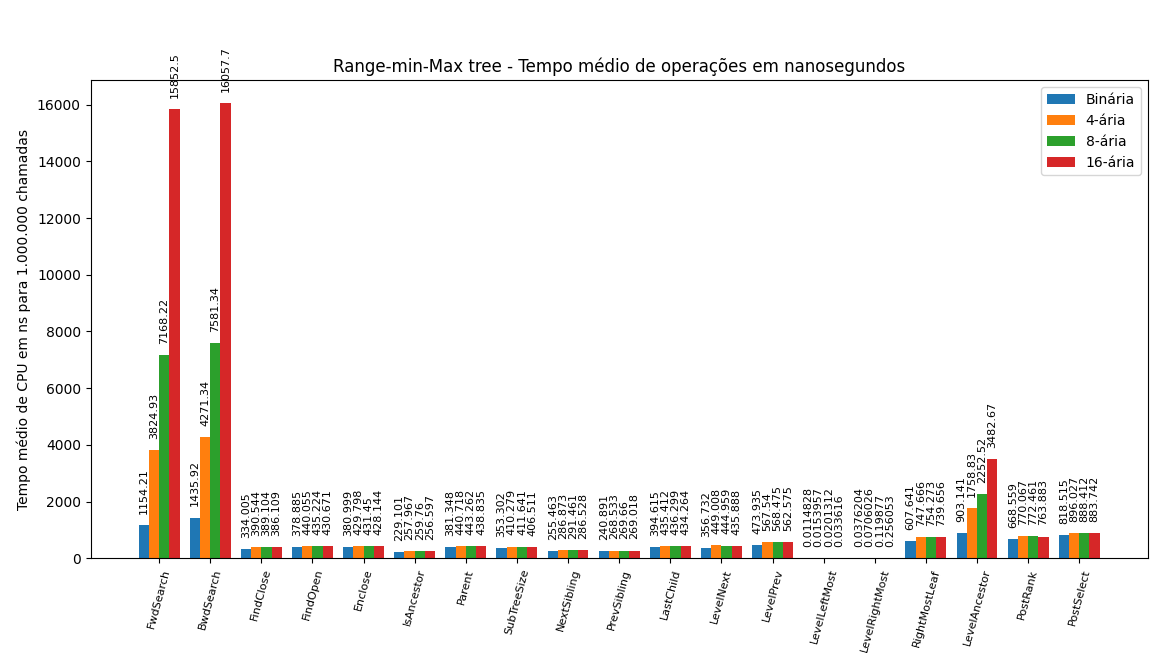
\includegraphics[scale=0.8]{images/ctree_i1000000.png}
        }
\end{figure}

\begin{figure}[!ht]
    \centering
      \caption[Operações sobre o conjunto de dado dna][Tempo médio de operações sobre o conjunto DNA]{
          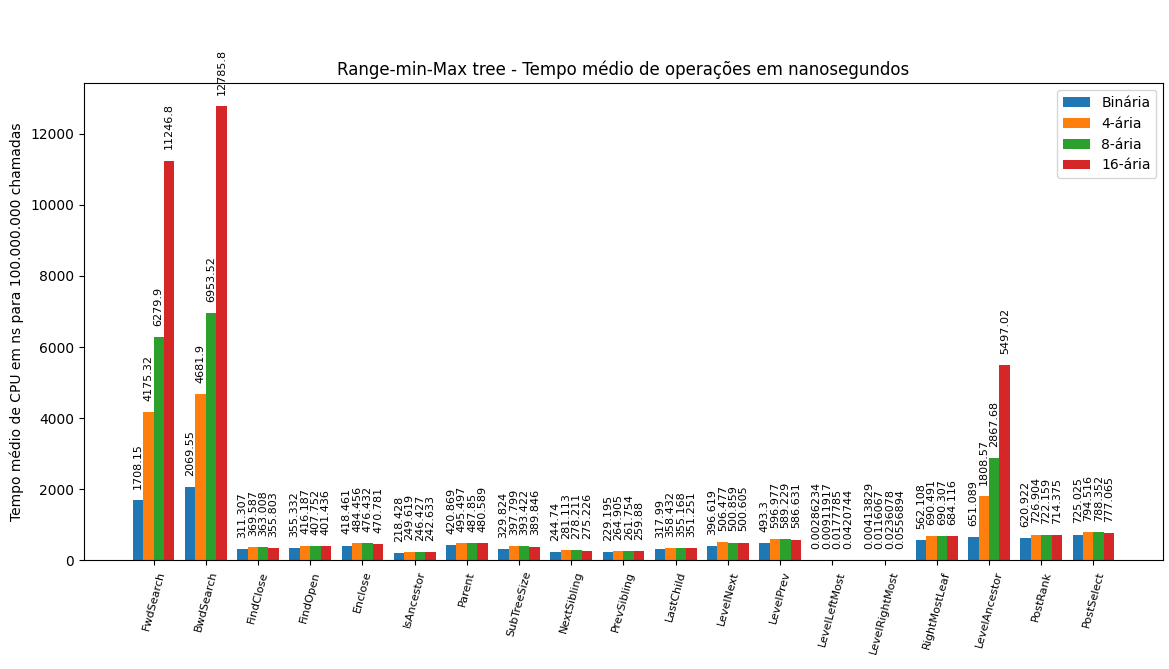
\includegraphics[scale=0.8]{images/dna_i100000000.png}
        }
\end{figure}

\begin{figure}[!ht]
    \centering
      \caption[Operações sobre o conjunto de dado proteins][Tempo médio de operações sobre o conjunto Proteins]{
          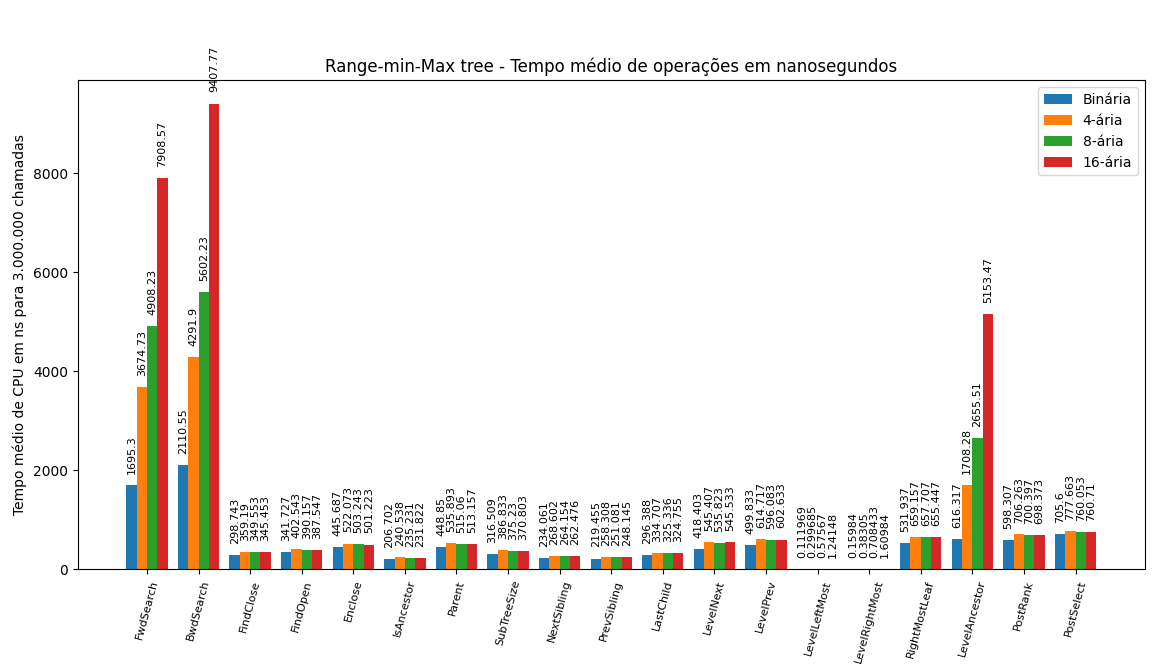
\includegraphics[scale=0.8]{images/prot_i3000000.png}
        }
\end{figure}

\begin{figure}[!ht]
    \centering
      \caption[Operações sobre o conjunto de dado wikipedia][Tempo médio de operações sobre o conjunto Wikipedia]{
          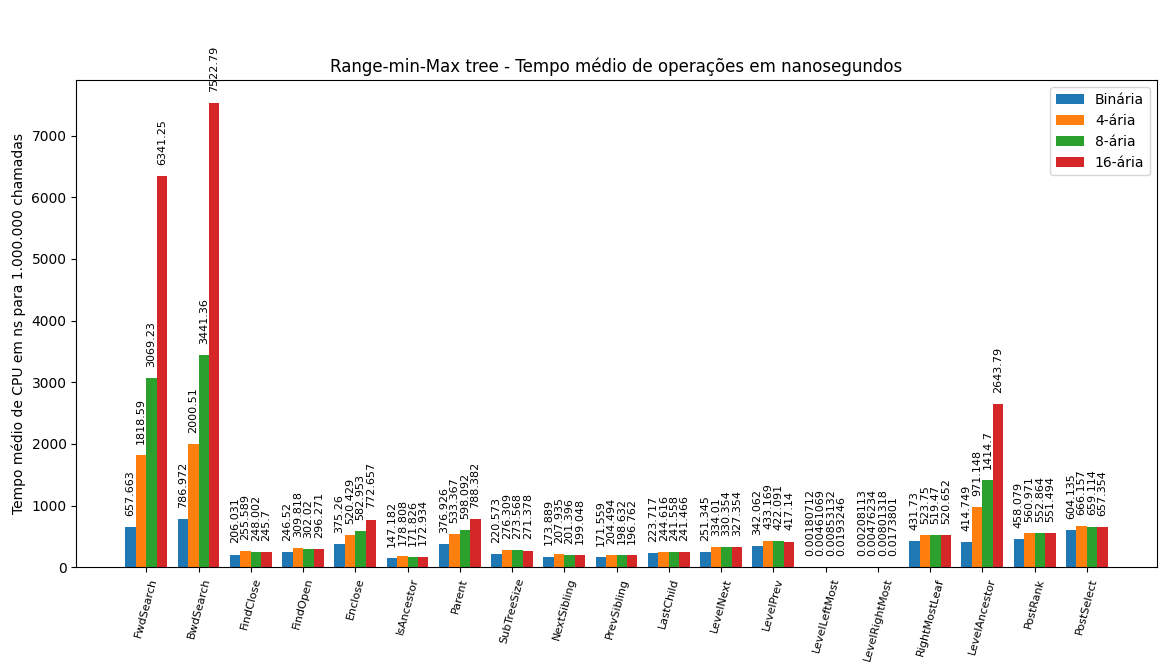
\includegraphics[scale=0.8]{images/wiki_i1000000.png}
        }
\end{figure}
\end{landscape}
%base de dados, configuração, experimentos, resultados
%figura, resultado destacado.